En la Figura~\ref{fig:model_loss} se muestra la el valor de la p\'erdida MSE~\eqref{eq:MSE} en funci\'on de la \'epoca de entrenamiento. \\

El mejor modelo de obtiene despu\'es de 89 \'epocas, con un valor de p\'erdida MSE para el conjunto de datos de entrenamiento de 8649.2, para el conjunto de datos de validaci\'on de 8411.9, y para el conjunto de datos de testeo de 9143.3. 

\begin{figure}[h]
\centering
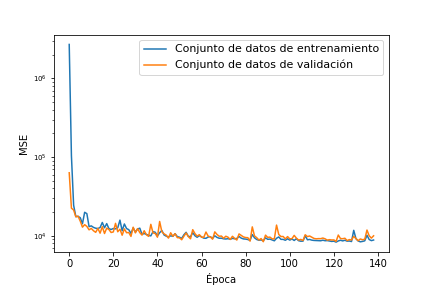
\includegraphics[width=0.75\textwidth]{figures/model_loss.png}
\caption{Valor del MSE en funci\'on de la \'epoca de entrenamiento para el conjunto de datos de entrenamiento (en azul) y para el conjunto de datos de validaci\'on (en naranja).}
\label{fig:model_loss}        
\end{figure}

En la Figura~\ref{fig:test_ptpred_tuneppt_genpt} se muestran sendas distribuciones bidimensionales del momento transverso de predicho por la red y del momento transverso dado por el algoritmo TuneP en funci\'on del momento transverso de generaci\'on para los muones del conjunto de datos de testeo. \\

\begin{figure}[h]
\centering
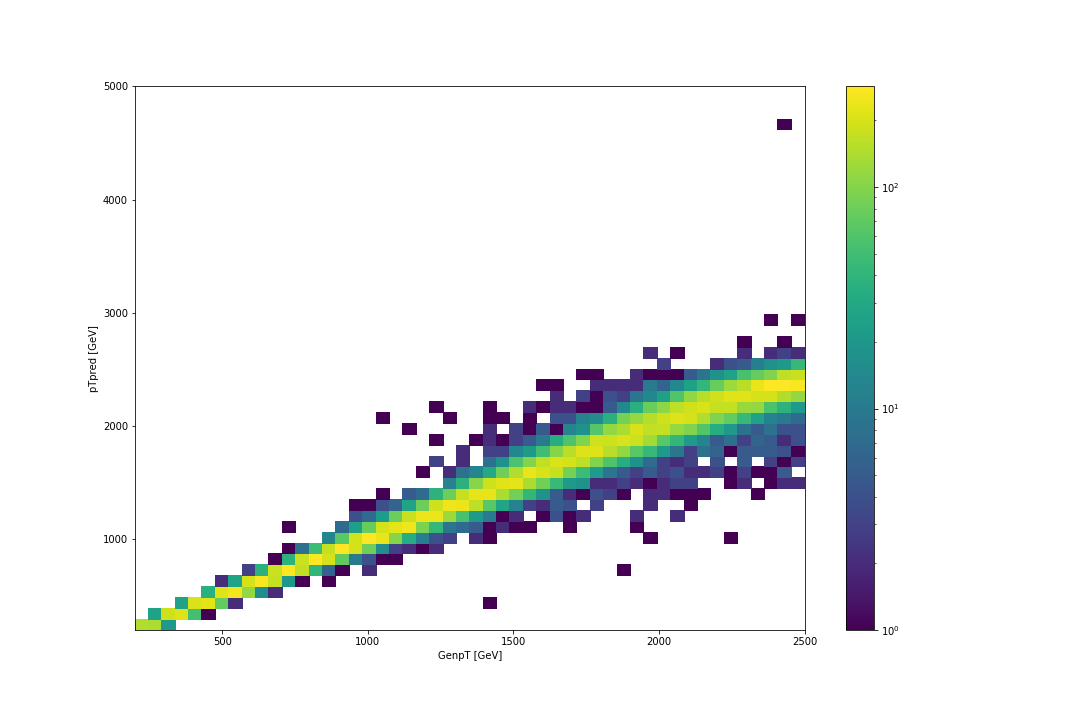
\includegraphics[width=1.0\textwidth]{figures/data_test_ptpred_genpt.png}
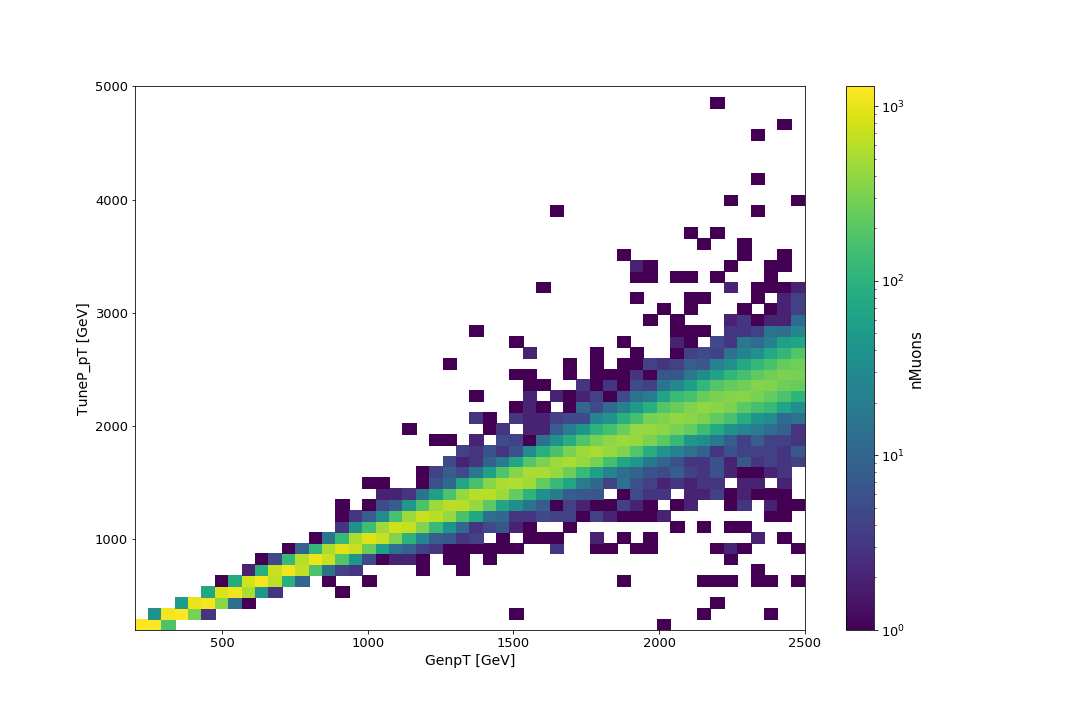
\includegraphics[width=1.0\textwidth]{figures/data_test_tuneppt_genpt.png}

\caption{Distribuci\'on bidimensional del $p_{T}$ en funci\'on del $p_{T}$ de generaci\'on para los muones del conjunto de datos de testeo. Arriba: $p_{T}$ predicho por la red neuronal en el eje de abscisas. Abajo: $p_{T}$ dado por el algoritmo TuneP en el eje de abscisas.}
\label{fig:test_ptpred_tuneppt_genpt}  
\end{figure}

Por otra parte, en la Figura~\ref{fig:R_vs_genpt} se muestra la dependencia del promedio y de la desviaci\'on est\'andar de la distribuci\'on de $R$ con el $p_{T}$ de generaci\'on para los muones del conjunto de datos de testeo, comparando en ambos casos los resultados que se obtienen al introducir en~\eqref{eq:R} el $p_{T}$ dado por el algoritmo TuneP, y el $p_{T}$ predicho por la DNN. \\
Se observa cualitativamente que la respuesta de la DNN es aproximadamente plana para los muones con $p_{T} > 1200$ GeV, mientras que cuando se toma el $p_{T}$ proporcionado por el algoritmo TuneP la asignaci\'on del momento transverso se va degradando progresivamente conforme aumenta el $p_{T}$ de generaci\'on. El hecho de que la resoluci\'on se aplane para valores altos del $p_{T}$ indica que la DNN es capaz de aprender la forma de las cascadas como funci\'on del momento transverso, reduciendo as\'i la dependencia natural del aumento en la resoluci\'on con el $p_{T}$ debida a la medida de saggita. \\

\begin{figure}[h]
\centering
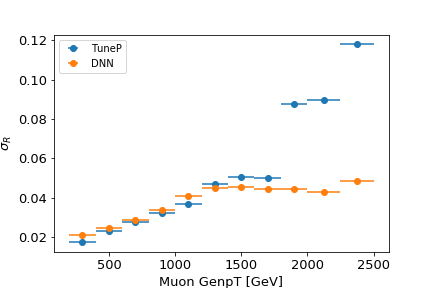
\includegraphics[width=0.7\textwidth]{figures/SigmaR_vs_genpT.png}
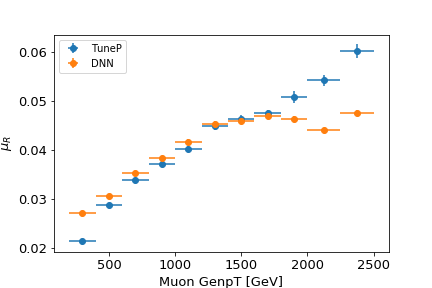
\includegraphics[width=0.7\textwidth]{figures/MeanR_vs_genpT.png}
\caption{Dependencia de la desviaci\'on est\'andar $\sigma$ (arriba) y de la media $\mu$ (abajo) de la variable $R$~\eqref{eq:R} con el $p_{T}$ generado. Ambas magnitudes se calculan a partir de la distribuci\'on de $R$ en cada bin de $p_{T}$. Azul: Tomando el $p_{T}$ proporcionado por el algoritmo TuneP en la definici\'on de $R$. Naranja: Tomando el $p_{T}$ predicho por la DNN en la definici\'on de $R$.}
\label{fig:R_vs_genpt}        
\end{figure}

A la hora de cuantificar los resultados obtenidos ha de tenerse en cuenta que la red ha sido alimentada con muones generados con un valor m\'aximo para el $p_{T}$ de 2500 GeV, por tanto es natural pensar que el modelo va a tender a asignar un momento transverso igual o menor a este valor m\'aximo a los muones cuyo $p_{T}$ sea cercano a 2500 GeV. Por este motivo, y para tener resultados m\'as coherentes, la evaluaci\'on del m\'etodo se har\'a con muones con momento transverso generado en el rango 1200 $\leq p_{T} \leq$ 2000 GeV. \\

Para este rango de $p_{T}$, se obtiene un valor para la desviaci\'on est\'andar de $R$ en el conjunto de muones de testeo de $\sigma_{R_{TuneP}}$ = 0.061 usando el $p_{T}$ del algoritmo TuneP, y de $\sigma_{R_{pred}}$ = 0.045 usando el $p_{T}$ predicho por el modelo de regresi\'on. Por tanto, el m\'etodo implementado en este trabajo consigue una mejora en la resoluci\'on de la asignaci\'on del momento transverso de un 26\% respecto al momento transverso proporcionado por CMS. \\

\clearpage
